
% The \phantomsection command is needed to create a link to a place in the document that is not a
% figure, equation, table, section, subsection, chapter, etc.
% https://tex.stackexchange.com/questions/44088/when-do-i-need-to-invoke-phantomsection
\phantomsection

\chapter{Offline Nanosatellite Task Scheduling}\label{chap:onts}

This chapter delves into the application area of the experiments conducted for this dissertation, specifically focusing on the Offline Nanosatellite Task Scheduling (ONTS) problem.
Over the past decade, nanosatellites have gained significant attention from both industry and academia, primarily due to their cost-effective development and launch processes~\cite{shiromaCubeSatsBrightFuture2011,luciaComputationalNanosatelliteConstellations2021,nagelNanosatellitesAppliedOptical2020,saeedCubeSatCommunicationsRecent2020}.
Despite these advantages, the limited computational and energy resources of nanosatellites present substantial challenges in mission planning.
Effective task scheduling is essential to optimize resource utilization, enhance data quality, and ensure mission success, thereby securing a return on investment.

The ONTS problem is critical for the efficient development, deployment, and operation of nanosatellites.
From launch to disposal, the ONTS problem must be solved repeatedly.
At every communication window, new schedules must be generated and deployed, and the optimal schedule is determined by an iterative procedure, exploring different sets of tasks to be performed in the schedule's timespan.
Given a nanosatellite and a collection of tasks, determining the schedule with maximum Quality of Service (QoS) is a combinatorial problem.
Mathematical formulations have been proposed for this problem, from Integer Programming (IP)~\cite{rigoTaskSchedulingOptimal2021} to Mixed Integer Linear Programming (MILP)~\cite{rigoNanosatelliteTaskScheduling2021,semanEnergyAwareTaskScheduling2022} and Continuous-Time techniques~\cite{camponogaraContinuoustimeFormulationOptimal2022}.
However, the NP-hard nature of the problem renders multiple executions of the optimization algorithms (e.g., for different task configurations) within the timespan of a communication window an efficiency challenge.

The following section will present the problem statement with a description of the factors that are taken into consideration.
Then, the MILP formulation of the problem, proposed by \citeonline{rigoNanosatelliteTaskScheduling2021}, is presented, which will be the basis for the experiments presented in Part~\ref{experiments-and-results}.

% The instances to be solved share common features.
% Beyond the problem structure, which remains unaltered, tasks, orbit information, and battery capacity can be understood as being randomly drawn from an unknown distribution at every communication window.
% This setup fits the context of primal heuristics based on 
% 
% It involves determining an optimal schedule for task execution that maximizes Quality-of-Service (QoS).
% This requires careful consideration of various factors, including task priority, minimum and maximum activation events, execution time frames, periods, and execution windows.
% Additionally, the constraints imposed by the satellite's power resources and the complexities of energy harvesting and management systems must be addressed.
% By solving the ONTS problem, we can significantly improve the operational efficiency and effectiveness of nanosatellite missions, ensuring their success and sustainability.


\section{Problem Statement}\label{sec:onts-problem-statement}

Nanosatellite scheduling problems involve making decisions regarding the start and finish times of each task.
These tasks often require periodic execution and must be scheduled during specific moments along the satellite's orbit.
In addition to temporal constraints, energy availability throughout the orbit is a crucial resource that must be taken into account.
Figure \ref{fig:example-scheduling} illustrates an example of optimal scheduling, where each job is represented by a different color, and the activation and deactivation of tasks are depicted as steps in the signal sequence.

\begin{figure}[h]
    \centering
    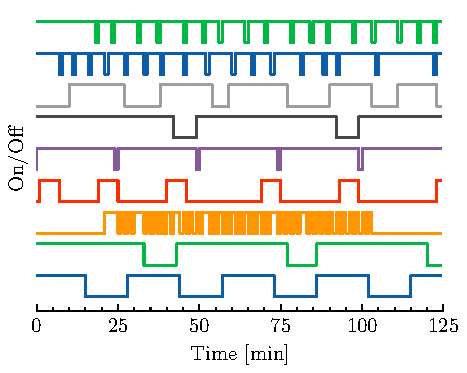
\includegraphics{schedule_example.pdf}
    \caption{Illustration of an optimum schedule for 9 tasks on a horizon of 125 time steps. Each color represents the executions of a different task.}
    \label{fig:example-scheduling}
\end{figure}

Effective scheduling must incorporate energy management to ensure that tasks do not consume more energy than the system can provide, thereby preventing the battery from depleting before the mission concludes.
Energy management is particularly challenging because the nanosatellite relies on solar panels for power.
The energy availability is influenced by the nanosatellite's attitude, which affects the orientation of the solar panels, and its trajectory relative to Earth's shadow, as depicted in Figure \ref{fig:onts-orbit}.
On top of that, the shared energy resources steps up the problem complexity, as each task's activation must be determined while taking into consideration the other tasks.

\begin{figure}[h]
    \centering
    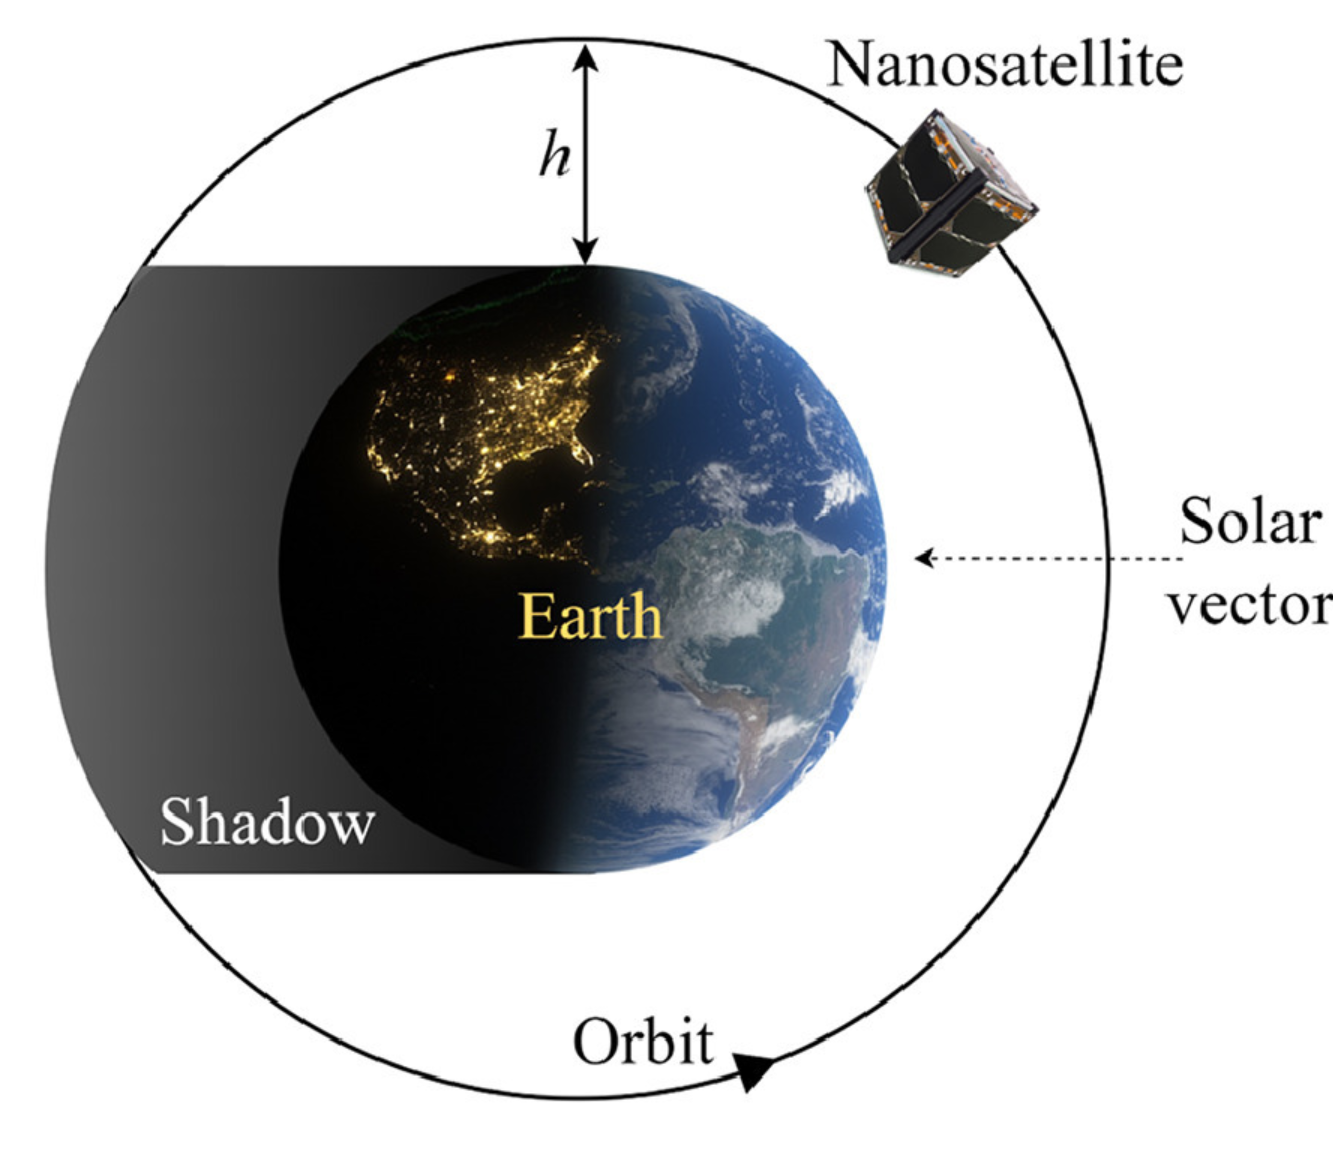
\includegraphics[width=0.5\textwidth]{onts_orbit.png}
    \caption{Illustration of a nanosatellite's orbit around Earth. Image from \citeonline{rigoBranchandpriceAlgorithmNanosatellite2022}.}
    \label{fig:onts-orbit}
\end{figure}

Instances of the ONTS problem are solved during the mission design phase, before launching the nanosatellite into orbit, and during the mission execution, at every communication window. 
During mission design, the instances are solved to evaluate the impact of the design choices in the nanosatellite capabilities.
During mission execution, the schedule is updated whenever possible to account for unexpected events (e.g., possible execution failures, hardware faults, unexpected battery drainage) or new requirements (e.g., new tasks, software updates).
More precisely, at every communication window, nanosatellite information (such as battery level, execution log, task results) is downloaded, the parameters of the ONTS problem are updated, a new schedule is generated, and the instructions are uploaded to the nanosatellite.


\section{MILP Formulation}\label{sec:onts-milp-formulation}

The formulation presented here was proposed by \citeonline{rigoTaskSchedulingOptimal2021} and the reader is advised to refer to the original work for further details.

Given a set $\mathcal{J}=\{1,...,J\}$ of tasks (or jobs), and a set $\mathcal{T}=\{1,...,T\}$ of time units of the scheduling horizon, let variables $x_{j,t}$ represent the allocation of task $j$ at time $t$, $\forall j\in \mathcal{J}, \forall t\in \mathcal{T}$.
Naturally, each $x_{j,t}$ is a binary variable, in which value $1$ indicates that task $j$ is scheduled to be in execution at time $t$.
When convenient, these variables will be represented as a vector \[
    % \bm{x}=(x_{1,1},\ldots,x_{1,T},\ldots,x_{J,1},\ldots,x_{J,T})
    \bm{x} = \left( x_{j,t} \right)_{\substack{j=1,\ldots,J\\ t=1,\ldots,T}}
,\] which is a notation also used for other variables and parameters.

Every task $j$ has an associated priority $u_j > 0$, such that the mission's QoS is defined as
\begin{equation}\label{eq:qos}
    {\rm QoS}(\bm{x};\bm{u}) = \sum_{j=1}^{J} \sum_{t=1}^{T} {u}_{j} x_{j,t}
.\end{equation}
As mentioned previously, the goal of the optimization problem is to find a schedule that maximizes the QoS.

Auxiliary variables $\phi_{j,t}$ are defined for every $j\in \mathcal{J}$ and $t\in \mathcal{T}$, which represent the startup of the task, i.e., $\phi_{j,t} = 1$ indicates that task $j$ is not running at time $t-1$ but its execution is started at time $t$.
The behavior of these auxiliary variables is ensured by
\begin{equation}\label{eq:phi-constraints}
    \begin{aligned}
	& \phi_{j,t} \geq x_{j,t}, &~\forall j\in\mathcal{J},\, t = 1  \\
        & \phi_{j,t} \geq x_{j,t} - x_{j,(t-1)}, &~\forall j\in\mathcal{J}, \,\forall t\in\mathcal{T}: t > 1   \\
        & \phi_{j,t} \leq x_{j,t}, &~\forall j\in\mathcal{J}, \,\forall t\in\mathcal{T}   \\
        & \phi_{j,t} \leq 2 - x_{j,t} - x_{j,(t-1)}, &~\forall j\in\mathcal{J}, \,\forall t\in\mathcal{T}: t > 1
    .\end{aligned}
\end{equation}

The multiple requirements of each task are ensured by a series of constraints.
Each task $j$ may run only during a specified time window delimited by $w_{j}^{\text{min}}$ and $w_{j}^{\text{max}}$, which is imposed by
\begin{equation}\label{eq:window-constraints}
    \begin{aligned}
        &\sum_{t=1}^{\textcolor{black}{w^{\min}_{j}}} x_{j,t} = 0,  & \forall j\in\mathcal{J} \\
        &\sum_{t=w^{\max}_{j}+1}^{T} x_{j,t} = 0, & \forall j\in\mathcal{J}
    .\end{aligned}
\end{equation}
Such constraints can be used to force a task to be executed when the nanosatellite is passing over a predetermined region.

To limit continuous executions, a task $j$ is constrained to run without interruption for least $t_j^{\text{min}}$, and at most $t_j^{\text{max}}$ time steps, which is imposed by
\begin{equation}\label{eq:execution-gap-constraints}
    \begin{aligned}
        &\sum_{l=t}^{t+{t}^{\min}_{j}-1} x_{j,l} \geq {t}^{\min}_{j} \phi_{j,t},  &\forall t \in \{1,...,T-{t}^{\min}_{j} + 1\}, \forall j\in\mathcal{J} \\
        &\sum_{l=t}^{t+{t}^{\max}_{j}} x_{j,l} \leq {t}^{\max}_{j},  &\forall t \in \{1,...,T-{t}^{\max}_{j}\}, \forall j\in\mathcal{J}
    .\end{aligned}
\end{equation}
Complementary, and having in mind that the end of schedule is not the end of the nanosatellite life, the addition of constraint
\begin{equation}\label{eq:execution-end-constraints}
    \begin{aligned}
        &\sum_{l=t}^{T} x_{j,l} \geq (T - t + 1) \phi_{j,t},  & \forall t \in \{T-{t}^{\min}_{j} + 2,...,T\}, \forall j\in\mathcal{J}
    \end{aligned}
\end{equation}
enables the start of the execution of a task close to the end of the schedule horizon, and keep it running until the end.

For a task to be executed periodically, at least every $p_j^{\text{min}}$ time steps, and at most every $p_j^{\text{max}}$ time steps, the following constraints are added:
\begin{equation}\label{eq:prediodicity-constraints}
    \begin{aligned}
        &\sum_{l=t}^{t+{p}^{\min}_{j}-1} \phi_{j,l} \leq 1,   & \forall t \in \{1,...,T-{p}^{\min}_{j}+1\}, \forall j\in\mathcal{J}  \\
        & \sum_{l=t}^{t+{p}^{\max}_{j}-1} \phi_{j,l} \geq 1,  & \forall t \in \{1,...,T-{p}^{\max}_{j}+1\},  \forall j\in\mathcal{J} 
    .\end{aligned}
\end{equation}
On top of that, a task may be required to run multiple times over the planning horizon.
The constraints
\begin{equation}\label{eq:multiple-execs-constraints}
    \begin{aligned}
        &\sum_{t=1}^{T} \phi_{j,t} \geq {y}^{\min}_{j}, &\forall j\in\mathcal{J}   \\
        &\sum_{t=1}^{T} \phi_{j,t} \leq {y}^{\max}_{j}, &\forall j\in\mathcal{J}
    \end{aligned}
\end{equation}
are added to ensure at least $y_{j}^{\text{min}}$ and at most $y_j^{\text{max}}$ runs are performed for task $j$.

The energy-management restrictions are ensured through multiple constraints.
Given $r_t$, the power available from the solar panels at each time $t$, $q_j$, the power required by each task $j$, and $\gamma~V_{b}$, the maximum power the battery can provide, then
\begin{equation}\label{eq:power-consumption-constraints}
    \begin{aligned}
	&\sum_{j=1}^{J} q_{j} x_{j,t} \leq r_t + \gamma~V_{b}, & \forall t\in\mathcal{T}
    \end{aligned}
\end{equation}
limits the power consumption to realistic levels.
Auxiliary variables $b_t$ and $\text{SoC}_t$ represent, resp., the exceeding power and the State of Charge (SoC) over each time $t\in \mathcal{T}$.
Given $Q$, the battery capacity, and $e$, the discharge efficiency, the exceeding power is ensured by
\begin{equation}\label{eq:exceeding-power-constraints}
    \begin{aligned}
	& b_{t} = r_{t} - \sum_{j \in \mathcal{J}} q_{j} x_{j,t}, &  \forall t \in \mathcal{T}
    ,\end{aligned}
\end{equation}
while the SoC is ensured by
\begin{equation}\label{eq:SoC-constraints}
    \begin{aligned}
    &\text{SoC}_{t+1} = \text{SoC}_{t} + \frac{b_{t}~e}{60~Q~V_{b}}, & \forall t \in \mathcal{T}  \\
    &\text{SoC}_{t} \leq 1, & \forall t\in\mathcal{T}    \\
    &\text{SoC}_{t} \geq \rho, & \forall t\in\mathcal{T}
    ,\end{aligned}
\end{equation}
where $\rho$ is the allowed lower limit for the battery, which is usually greater than zero for safety purposes.

Finally, the ONTS problem is formulated as an MILP
\begin{equation}\label{eq:onts-milp}
\begin{aligned}
    \max_{\bm{x},\bm{\phi},\bm{\text{SoC}},\bm{b}} \quad & \eqref{eq:qos} \\
    \textrm{s.t.} \quad & (\ref{eq:phi-constraints} \text{--} \ref{eq:SoC-constraints}) \\
	    & x_{j,t}, \phi_{j,t} \in \left\{ 0,1 \right\} ,\quad \forall j\in \mathcal{J}, t\in \mathcal{T}
.\end{aligned} \tag{ONTS}
\end{equation}
Note that the constraints \eqref{eq:exceeding-power-constraints} and \eqref{eq:SoC-constraints} imply that the continuous variables $\bm{b}$ and $\bm{\text{SoC}}$ are uniquely determined by a given assignment for the binary variables $\bm{x}$ and $\bm{\phi}$.
Therefore, the problem can be reduced to finding an assignment $\bm{y}=(\bm{x},\bm{\phi}) \in \left\{ 0,1 \right\}^{n}$, where $n=2JT$.

Let $\mathcal{I}$ be the space of all MILP problems of the form \eqref{eq:onts-milp}.
Any instance $I\in \mathcal{I}$ is parameterized by $\pi_I = \left( \bm{u}, \bm{q}, \bm{y}^{\min}, \bm{y}^{\max}, \bm{t}^{\min}, \bm{t}^{\max}, \bm{p}^{\min}, \bm{p}^{\max}, \bm{w}^{\min}, \bm{w}^{\max}, \bm{r}, \rho, e, Q, \gamma, V_b \right) $, and, implicitly, by the number of tasks $J$ and the number of time units $T$.
Let $\Pi^{J,T}$ denote the space of parameter vectors as above, such that any instance $I\in \mathcal{I}$ can be uniquely determined by a parameter vector $\pi_{I}$ (given adequate $J$ and $T$).


